% Current Chinese manuscript: deterministic relative propagation response.
\section{接收模型与定位方法}\label{sec:current-model}
\subsection{传播响应与未知源系数}
考虑四个同步单天线接收站和两个静止辐射源。站位置$\mathbf r_\ell$已知，源位置$\mathbf p_k$待估，传播速度$c=3\times10^8$ m/s，传播距离和时延分别为
\begin{equation}
d_\ell(\mathbf p)=\|\mathbf p-\mathbf r_\ell\|_2,\qquad
\tau_\ell(\mathbf p)=d_\ell(\mathbf p)/c.
\end{equation}
在直达自由空间传播条件下，固定载频对应的公共场幅度常数并入源波形，站间相对幅度与$1/d_\ell$成正比。本模型使用基带时延，不另设站间载波相位或随机复衰减。位置、源波形及发射功率未知，站间相对响应由候选位置确定。

采用忽略观测窗边缘效应的频域近似模型\cite{ref05,ref04}。保留全部$M=N$个DFT频点，令$f_m$为有符号基带频率，$\mathbf x_m\in\mathbb C^L$为第$m$个频点的多站观测，定义
\begin{equation}\label{eq:new-response}
a_{\ell m}(\mathbf p)=\frac{e^{-j2\pi f_m d_\ell(\mathbf p)/c}}{d_\ell(\mathbf p)},\quad
\mathbf q_m(\mathbf p)=\frac{\mathbf a_m(\mathbf p)}{\|\mathbf a_m(\mathbf p)\|_2},\quad
\mathbf Q_m(\theta)=[\mathbf q_m(\mathbf p_1),\mathbf q_m(\mathbf p_2)].
\end{equation}
接收模型写为
\begin{equation}\label{eq:new-model}
\mathbf x_m=\mathbf Q_m(\theta)\mathbf s_m+\mathbf n_m,\qquad
\theta=[\mathbf p_1^T,\mathbf p_2^T]^T\in\mathbb R^4,\quad
\mathbf n_m\sim\mathcal{CN}(\mathbf0,\sigma_f^2\mathbf I_L).
\end{equation}
其中$\mathbf s_m$包含发射功率、初相及响应列的公共尺度。对响应列归一化只改变系数表示，不改变其列空间。仿真生成时对每个源的全部站观测施加同一个功率尺度，以固定全网平均接收功率；估计时保留接收数据的原始站间幅度，不进行逐站RMS归一化。以上三种尺度处理分别作用于传播常数、源功率和字典列。

\subsection{由似然到联合最小二乘}
在式\eqref{eq:new-model}下，各站及频点噪声独立。去除与参数无关的常数，负对数似然为
\begin{equation}
\mathcal L(\theta,\{\mathbf s_m\})=\sigma_f^{-2}\sum_m\|\mathbf x_m-\mathbf Q_m(\theta)\mathbf s_m\|_2^2.
\end{equation}
固定位置后，波形系数的最小范数LS解为
\begin{equation}\label{eq:2.8}
\widehat{\mathbf s}_m=\mathbf Q_m^\dagger\mathbf x_m.
\end{equation}
代回得到集中目标及其能量归一化形式：
\begin{equation}\label{eq:new-joint}
J(\theta)=\sum_m\|\mathbf P_m^\perp(\theta)\mathbf x_m\|_2^2,\qquad
\bar J(\theta)=\frac{J(\theta)}{E_x},\quad
\mathbf P_m^\perp=\mathbf I-\mathbf Q_m\mathbf Q_m^\dagger,\quad
E_x=\sum_m\|\mathbf x_m\|_2^2.
\end{equation}
$E_x$对给定观测为常数，归一化不改变最优位置：
\begin{equation}\label{eq:2.7}
\widehat\theta=\arg\min_{\theta\in\Omega^2}\bar J(\theta),\qquad\Omega=[-1000,1000]^2\ \mathrm{m}^2.
\end{equation}
双源求解是四个实位置参数的非凸优化；位置确定后，全部频点的源系数均可解析消去。

若只拟合一个候选源，利用$\|\mathbf q_m\|_2=1$，有
\begin{equation}\label{eq:new-ls-spectrum}
\min_{\{s_m\}}\sum_m\|\mathbf x_m-\mathbf q_m(\mathbf p)s_m\|_2^2
=E_x-S_{\mathrm{LS}}(\mathbf p),\qquad
S_{\mathrm{LS}}(\mathbf p)=\sum_m|\mathbf q_m^H(\mathbf p)\mathbf x_m|^2.
\end{equation}
这给出本轮的单源LS扫描谱。若另将补偿时延后的站间响应方向设为未知单位向量$\mathbf b$，则消元后需最大化$\mathbf b^H\mathbf R(\mathbf p)\mathbf b$，其解为$\lambda_{\max}(\mathbf R(\mathbf p))$。本轮响应方向已经由位置确定，因此使用式\eqref{eq:new-ls-spectrum}的匹配能量。特征分解用于下述MUSIC的子空间估计。

\subsection{方法对应关系与求解流程}\label{sec:new-methods}
表\ref{tab:new-methods}列出八种方法的评分和实际求解方式。各方法使用相同观测、已知站址、源数及搜索区域；连续位置均限制在$[-1000,1000]^2$ m内。
\begin{table}[htbp]\centering\small
\caption{比较方法及其与接收模型的关系}\label{tab:new-methods}
\begin{tabularx}{\linewidth}{lY{.8}Y{1.2}}\toprule
方法 & 目标或评分 & 求解方式\\\midrule
LS双峰 & 单源匹配能量 & 全区域扫描、取两个峰、逐峰精修\\
宽带MUSIC & 噪声子空间投影能量倒数 & 分段协方差、跨频聚合、取峰精修\\
已知响应MVDR & 跨频平均Capon功率 & 对角加载、取峰精修\\
AP & 联合残差下降量 & 条件投影、全区域候选、逐源交替更新\\
块NOMP & 残差匹配能量及联合LS & 逐源检测、二维Newton与循环更新\\
SBL-PDL-known & 稀疏贝叶斯证据 & 共享稀疏先验、后验更新、位置细化\\
多初值联合优化 & 四维集中LS & 谱候选与Sobol初值、连续联合优化\\
GA联合优化 & 四维集中LS & 实数编码遗传搜索、预算内联合精修\\\bottomrule
\end{tabularx}
\end{table}

\subsubsection{协方差空间谱}
将单次观测划分为$J_s$段，每段长$M_s=N/J_s$。在相同段内频率$f$上计算
\begin{equation}
\widehat{\mathbf R}_f=\frac1{J_s}\sum_{j=1}^{J_s}\mathbf x_{f,j}\mathbf x_{f,j}^H.
\end{equation}
MUSIC对$\widehat{\mathbf R}_f$作特征分解，取最小的$L-K$个特征值所对应的特征向量组成$\mathbf E_{n,f}$。本轮采用跨频平均投影能量的倒数：
\begin{equation}\label{eq:new-music}
S_{\mathrm{MUSIC}}(\mathbf p)=\left[\frac1{M_s}\sum_f
\mathbf q_f^H(\mathbf p)\mathbf E_{n,f}\mathbf E_{n,f}^H\mathbf q_f(\mathbf p)\right]^{-1}.
\end{equation}
该式采用多源DPD的子空间思路\cite{ref04}，每段频率响应按段长重新构造。已知响应MVDR先计算各频点的Capon功率\cite{ref15}，再跨频平均：
\begin{equation}\label{eq:new-mvdr}
\widetilde{\mathbf R}_f=\widehat{\mathbf R}_f+eta\frac{\operatorname{tr}(\widehat{\mathbf R}_f)}L\mathbf I,
\qquad S_{\mathrm{MVDR}}(\mathbf p)=\frac1{M_s}\sum_f
\left[\mathbf q_f^H(\mathbf p)\widetilde{\mathbf R}_f^{-1}\mathbf q_f(\mathbf p)\right]^{-1}.
\end{equation}
这里$\eta=10^{-3}$，响应向量已知。DPD-HR\cite{ref06}是相关的高分辨率直接定位研究，其未知响应方向下的谱构造与式\eqref{eq:new-mvdr}有所区别。MUSIC和MVDR分别采用4段和8段，均只使用当前记录；估计包括全部段内DFT频点。

\subsubsection{条件投影与AP}
固定其他源的位置，记其响应矩阵为$\mathbf B_m$，并令
\begin{equation}
\mathbf P_{B,m}^\perp=\mathbf I-\mathbf B_m\mathbf B_m^\dagger,\quad
\mathbf r_m=\mathbf P_{B,m}^\perp\mathbf x_m,\quad
\mathbf u_m(\mathbf p)=\mathbf P_{B,m}^\perp\mathbf q_m(\mathbf p).
\end{equation}
同时投影观测与候选响应，再消去当前源系数，可得新增候选带来的残差下降：
\begin{equation}\label{eq:new-conditional}
S_{\mathrm{cond}}(\mathbf p\mid\mathbf B)=\sum_m
\frac{|\mathbf u_m^H(\mathbf p)\mathbf r_m|^2}{\mathbf u_m^H(\mathbf p)\mathbf u_m(\mathbf p)},\qquad
J([\mathbf B,\mathbf p])=J(\mathbf B)-S_{\mathrm{cond}}(\mathbf p\mid\mathbf B).
\end{equation}
当$\mathbf u_m=0$时该项增量为零。AP从LS谱候选开始，逐源扫描该条件评分，保留多个候选作连续精修，每次位置更新后重新拟合全部源系数。循环中穿插全区域重新搜索，剩余时间用于更细网格的候选补充。它与固定其他源波形后直接相减的更新不同：投影步骤同步重新消除了其他源的系数。

\subsubsection{块NOMP与联合优化}
块NOMP借鉴连续参数检测和循环精修\cite{ref08}，将每个源的各频点系数组成一个块。新增源通过残差上的$\sum_m|\mathbf q_m^H\mathbf r_m|^2$检测；源数固定为$K$。循环更新第$k$个源时，先由联合拟合重建其余源并相减，得到$\mathbf e_{k,m}=\mathbf x_m-\sum_{j\ne k}\mathbf q_m(\mathbf p_j)\widehat s_{j,m}$。局部目标为$-E_x^{-1}\sum_m|\mathbf q_m^H(\mathbf p)\mathbf e_{k,m}|^2$，使用二维阻尼Newton方向
\begin{equation}
\Delta\mathbf p=-(\mathbf H+\lambda\mathbf I)^{-1}\mathbf g,
\end{equation}
其中$\mathbf g$和$\mathbf H$为当前局部目标的梯度和Hessian，$\lambda$使修正后的Hessian正定。步长上限为50 m，回溯接受下降步；每次加入源后循环更新各位置及全部波形系数。该实现将NOMP的连续精修用于二维传播字典。

多初值方法直接最小化式\eqref{eq:new-joint}，初值由LS谱候选与Sobol点组成，逐个执行四维L-BFGS-B。GA采用相同目标和位置边界，用谱候选与Sobol点构造实数编码种群，执行锦标赛选择、模拟二进制交叉\cite{ref16}和多项式变异，并保留精英个体。若预算允许，末尾对最优个体进行联合连续精修。这两类方法提供了与逐源更新不同的联合搜索路径。

\subsubsection{共享稀疏先验与位置细化}
SBL-PDL-known采用位置参数化字典$\mathbf A_m=[\mathbf q_m(\mathbf z_1),\ldots,\mathbf q_m(\mathbf z_G)]$和跨频共享先验$\mathbf s_m\sim\mathcal{CN}(\mathbf0,\Gamma)$，其中$\Gamma=\operatorname{diag}(\gamma_1,\ldots,\gamma_G)$。令
\begin{align}
\mathbf C_m&=\sigma_f^2\mathbf I+\mathbf A_m\Gamma\mathbf A_m^H,\\
\mu_m&=\Gamma\mathbf A_m^H\mathbf C_m^{-1}\mathbf x_m,\qquad
\Sigma_m=\Gamma-\Gamma\mathbf A_m^H\mathbf C_m^{-1}\mathbf A_m\Gamma,\\
\gamma_i^{\mathrm{new}}&=\frac1M\sum_m\bigl(|\mu_{i,m}|^2+[\Sigma_m]_{ii}\bigr).
\end{align}
随后对选中的$K$个活动位置作局部更新，要求证据目标
\begin{equation}\label{eq:new-evidence}
\mathcal E(\mathbf z,\Gamma)=\sum_m\left[\log\det\mathbf C_m+\mathbf x_m^H\mathbf C_m^{-1}\mathbf x_m\right]
\end{equation}
下降，位置移动限制在当前网格点的半网格邻域内。这里借鉴参数化字典学习\cite{ref13}，采用确定性相对响应，故记为SBL-PDL-known。空间图展示$M^{-1}\sum_m|\mu_{i,m}|^2$，与包含后验方差的超参数更新量分别定义。

\begin{figure}[htbp]\centering
\begin{tikzpicture}[>=Stealth,node distance=5mm, every node/.style={font=\small}, box/.style={draw,rounded corners,align=center,minimum height=10mm,text width=30mm}]
\node[box] (x) {多站混合观测\\频域响应};
\node[box,right=of x] (s) {空间谱候选\\或全局初值};
\node[box,right=of s] (p) {位置搜索\\与连续精修};
\node[box,right=of p] (w) {联合波形拟合\\评价残差};
\draw[->] (x)--(s);\draw[->](s)--(p);\draw[->](p)--(w);
\draw[->](w.south)--++(0,-.65)-|node[pos=.25,below]{AP、块NOMP及联合LS求解器的循环更新}(p.south);
\end{tikzpicture}
\caption{联合LS方法的数据流。协方差空间谱与SBL分别使用其自身评分和更新目标。}\label{fig:new-flow}
\end{figure}

\subsection{位置导数、局部信息与曲率}
令$\mathbf v_\ell=(\mathbf p-\mathbf r_\ell)/d_\ell$。对位置求导有
\begin{equation}
\nabla_{\mathbf p}a_{\ell m}=a_{\ell m}\left(-\frac1{d_\ell}-j\frac{2\pi f_m}{c}\right)\mathbf v_\ell,\qquad
\partial_i\mathbf q_m=\frac{\partial_i\mathbf a_m}{h_m}-\frac{\mathbf a_m\operatorname{Re}(\mathbf a_m^H\partial_i\mathbf a_m)}{h_m^3},
\quad h_m=\|\mathbf a_m\|_2.
\end{equation}
记$\mathbf H_m=\partial(\mathbf Q_m\mathbf s_m)/\partial\theta^T$，求导时固定系数。在响应局部满列秩、噪声方差已知的条件下，消去未知复波形后的位置信息为\cite{ref05,ref10}
\begin{equation}\label{eq:new-information}
\mathbf I_{\theta}^{\mathrm{eff}}=\frac{2}{\sigma_f^2}\operatorname{Re}\sum_m\mathbf H_m^H\mathbf P_m^\perp\mathbf H_m.
\end{equation}
响应列缩放引入的导数分量位于响应列空间内，经$\mathbf P_m^\perp$消除后，原始响应和归一化响应给出一致的位置信息。弱源能量、源间响应相似性与几何条件共同影响局部曲率。

无噪声且模型正确时，若消元后实残差的有效Jacobian满列秩，则真值处LS Hessian正定，并存在局部强凸邻域。有噪声时Hessian还包含残差相关项，真值一般也不是样本目标的驻点。因此，局部信息描述精度和耦合，有限时间内能否进入有效邻域还取决于候选覆盖和搜索路径。附录\ref{sec:2}保留条件评分上界、窄峰近似及强源误差残留的补充推导。

\section{仿真验证与分析}\label{sec:new-results}
\subsection{信号、样本与比较条件}
四站坐标为$(500,0)$、$(0,500)$、$(-500,0)$、$(0,-500)$ m。两个源独立位于$[-1000,1000]^2$ m内，源到各站距离至少150 m，源间距至少300 m。正式比较包含12个独立布局，每个布局使用一组基础波形和噪声，在六档功率差下重复使用。

信号为根升余弦成形的BPSK，符号率10 MHz、滚降系数0.25、带宽12.5 MHz，采样率100 MHz，记录长度$N=16384$，观测时长163.84 $\mu$s。两源均为零中心频率，频谱完全重叠。时域复噪声方差为1；DFT按$1/N$归一化后$\sigma_f^2=1/N$。弱源全网平均带内SNR固定为6 dB，对应全带SNR约$-3.03$ dB。只增加强源功率，定义
\begin{equation}
\gamma=\frac{\overline P_{\mathrm{weak}}}{\overline P_{\mathrm{strong}}},\qquad
\Delta P=-10\log_{10}\gamma\in\{0,3,6,9,12,15\}\ \mathrm{dB}.
\end{equation}
功率均指不含噪声的全网平均接收功率。0 dB沿用固定源身份统计强、弱源，以保持配对关系。

弱源功率通过独立开发样本上的30 s单源AP校准：16个布局、每布局2次实现，3 dB和6 dB条件下分别有26/32、31/32条记录达到20 m判据；6 dB为满足30/32准则的首个测试档位。正式数据包含72条混合观测、12条孤立弱源观测和72条孤立强源观测。每条混合观测都具有相同信号分量和噪声的单源参照；孤立弱源在六档间复用。每种方法处理156条观测，八种方法共1248项任务。

\begin{table}[htbp]\centering\small
\caption{实际求解参数}\label{tab:new-config}
\begin{tabularx}{\linewidth}{lY{1}}\toprule
方法 & 参数\\\midrule
LS双峰 & 10 m网格，前5个候选，逐峰Powell精修\\
MUSIC / MVDR & 20 m网格；分别4段、8段；MVDR相对加载$10^{-3}$\\
AP & 初始20 m网格、前10候选、5轮循环；第2、4轮全域回访，预算内继续10 m和5 m搜索\\
块NOMP & 10 m检测网格；每次增加源后5轮循环，局部Newton最多3步\\
SBL-PDL-known & 50 m字典网格、最多50轮；活动位置每次最多3次局部迭代，频点分块256\\
多初值联合优化 & 20 m候选网格、32组初值，每组最多60次联合优化迭代\\
GA联合优化 & 种群64、精英4、三元锦标赛；交叉概率0.9、分布指数15；每维变异概率0.25、分布指数20；最多200代，15代无改进停止\\\bottomrule
\end{tabularx}
\end{table}
混合场景每次预算60 s，单源场景30 s，计时包括预处理、数据传输和求解。计算采用双精度复数及RTX 4070 Ti SUPER。5、15、30、60 s节点只读取节点前已保存的估计；提前完成的方法沿用最终输出。完整耗时包含退出检查的少量开销，因而可能略超过设定预算。全部任务完成，未出现数值失败。

\subsection{评价指标}
成功率使用20 m门控的一对一匹配：先最大化门内匹配数，再最小化匹配平方距离。分别统计强源、弱源和双源同时成功率。RMSE和CDF使用未截断平方距离和最小的一对一匹配，并包含大误差样本。两种匹配分别用于阈值判定和误差统计。

集合误差采用GOSPA\cite{ref12}，$p=2$、$c_0=100$ m、$\alpha=2$。对部分匹配$\mathcal A$，其平方形式为
\begin{equation}
d_{\mathrm{GOSPA}}^2=\min_{\mathcal A}\left\{\sum_{(i,j)\in\mathcal A}\|\mathbf p_i-\widehat{\mathbf p}_j\|^2+
\frac{c_0^2}{2}\left(K+\widehat K-2|\mathcal A|\right)\right\}.
\end{equation}
$c_0$控制集合误差的截断，20 m控制成功判据。混合数据最终均有双源输出；时间节点上尚无输出的任务仍计入成功率分母。跨功率档汇总的72条记录来自12个重复使用的布局。

\subsection{功率差与定位表现}
\begin{table}[htbp]\centering\small\setlength{\tabcolsep}{4pt}
\caption{60 s节点的混合源定位结果（每种方法72条记录）}\label{tab:g10-summary}
\begin{tabular}{lrrrrrr}\toprule
方法 & 强源成功 & 弱源成功 & 双源成功 & 强源RMSE/m & 弱源RMSE/m & 均值耗时/s\\\midrule
LS双峰 & 65 & 7 & 3 & 321.89 & 1054.78 & 2.72\\
宽带MUSIC & 18 & 7 & 1 & 218.45 & 1063.95 & 0.55\\
已知响应MVDR & 51 & 14 & 9 & 214.66 & 983.95 & 0.58\\
AP & 68 & 58 & 55 & 8.48 & 17.80 & 60.05\\
块NOMP & 63 & 41 & 36 & 152.37 & 307.52 & 8.70\\
SBL-PDL-known & 21 & 4 & 0 & 428.79 & 1131.52 & 51.34\\
多初值联合优化 & 59 & 14 & 12 & 169.51 & 917.28 & 60.06\\
GA联合优化 & 44 & 11 & 5 & 117.85 & 806.31 & 60.18\\
\bottomrule\end{tabular}
\end{table}
\begin{figure}[htbp]\centering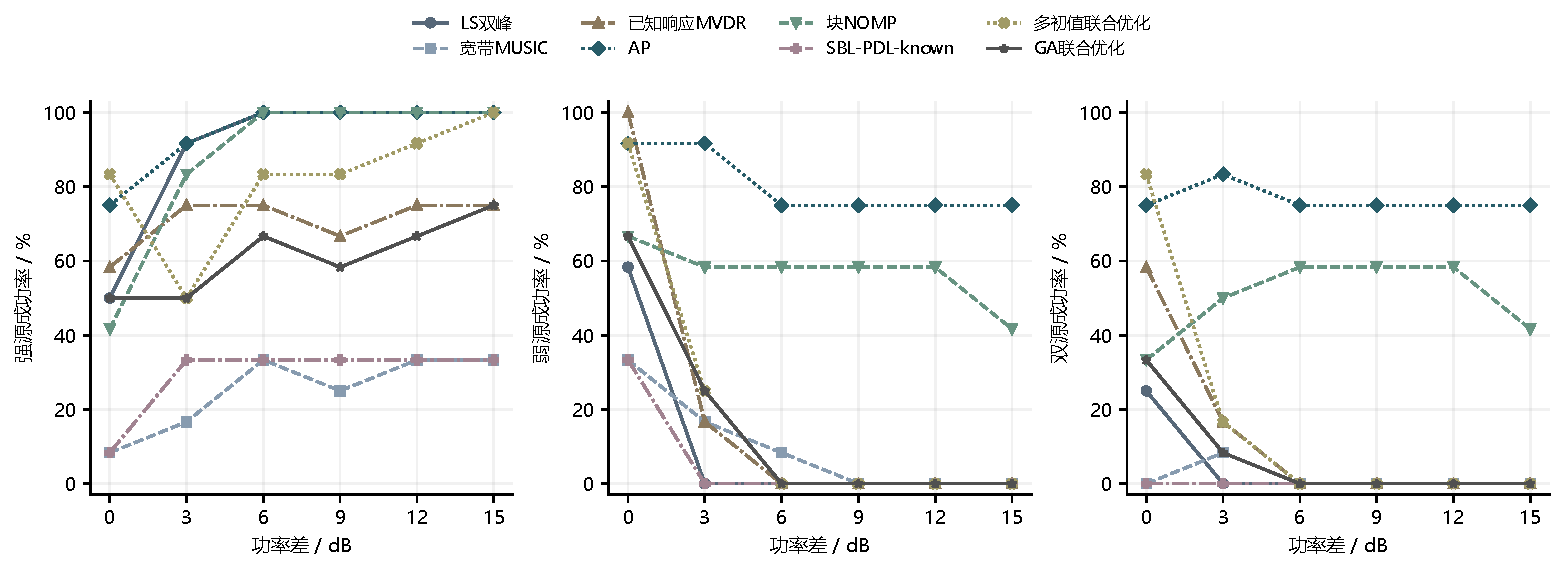
\includegraphics[width=\linewidth]{figures/g10_success.pdf}
\caption{60 s节点的强源、弱源及双源成功率。每档12个布局，成功阈值20 m。}\label{fig:g10-success}\end{figure}
表\ref{tab:g10-summary}和图\ref{fig:g10-success}显示，AP的弱源与双源成功数分别为58/72和55/72，弱源RMSE为17.80 m。其弱源成功数随功率差依次为11、11、9、9、9、9；在6--15 dB区间保持相同成功数。块NOMP对应为8、7、7、7、7、5，汇总弱源成功41/72。LS双峰、MUSIC、MVDR、SBL及两种通用联合优化在较大功率差下的弱源成功数明显下降。对这些数据，候选检测后充分利用联合拟合的逐源更新较为有效。

\begin{figure}[htbp]\centering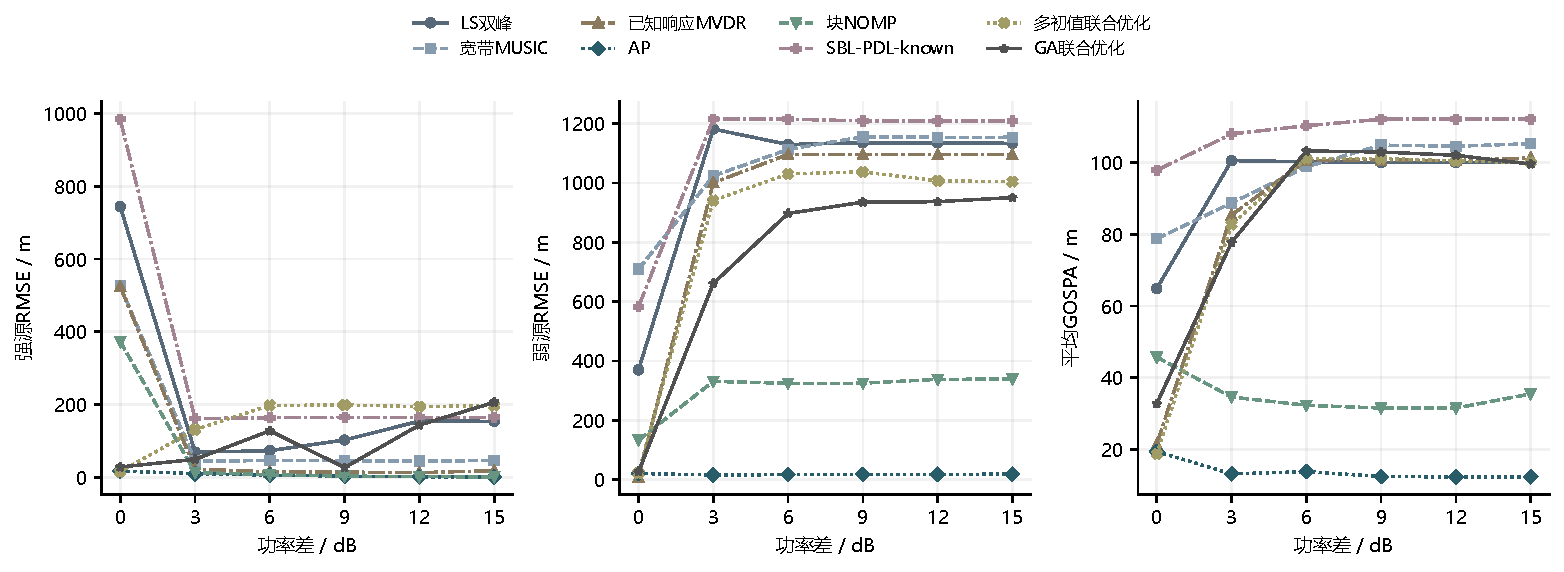
\includegraphics[width=\linewidth]{figures/g10_error.pdf}
\caption{强、弱源未截断RMSE及平均GOSPA随功率差的变化。}\label{fig:g10-error}\end{figure}
成功率与RMSE反映不同误差特征。块NOMP弱源成功率高于其余六种方法，但弱源RMSE为307.52 m，95\%误差分位约1027.47 m，仍有明显长尾。AP弱源95\%误差分位为45.12 m，最大误差为66.21 m。图\ref{fig:g10-cdf-strong}和图\ref{fig:g10-cdf-weak}展示六档功率差下的全部样本分布，避免仅用平均误差掩盖少量严重误定位。
\begin{figure}[htbp]\centering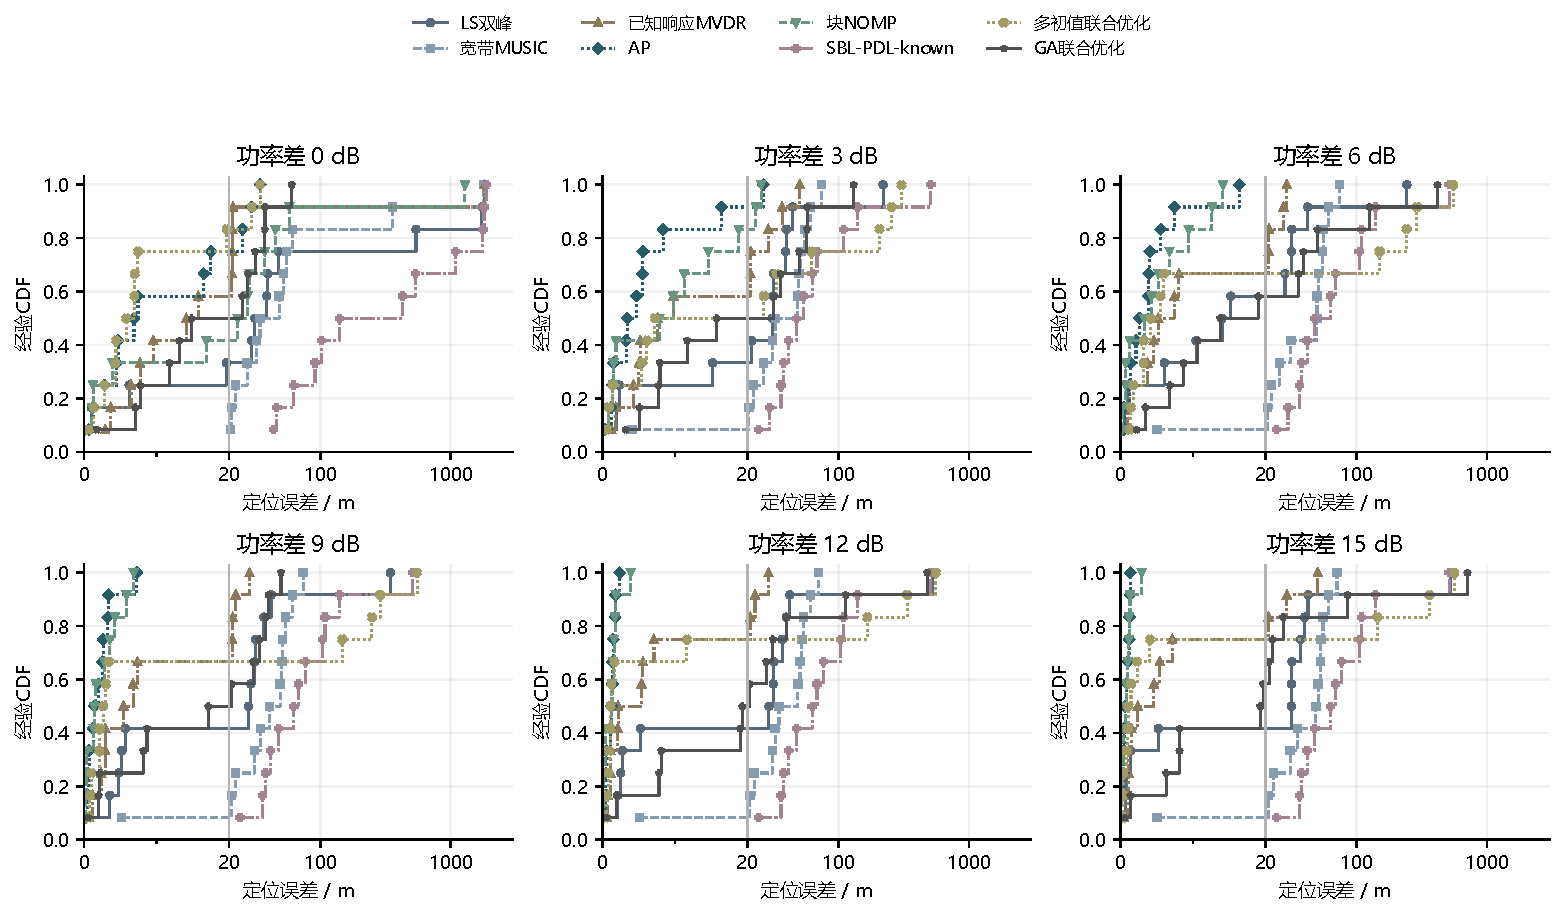
\includegraphics[width=\linewidth]{figures/g10_cdf_strong.pdf}
\caption{强源误差CDF。横轴在0--20 m线性显示，20 m以上采用对数尺度；每条曲线包含12条记录。}\label{fig:g10-cdf-strong}\end{figure}
\begin{figure}[htbp]\centering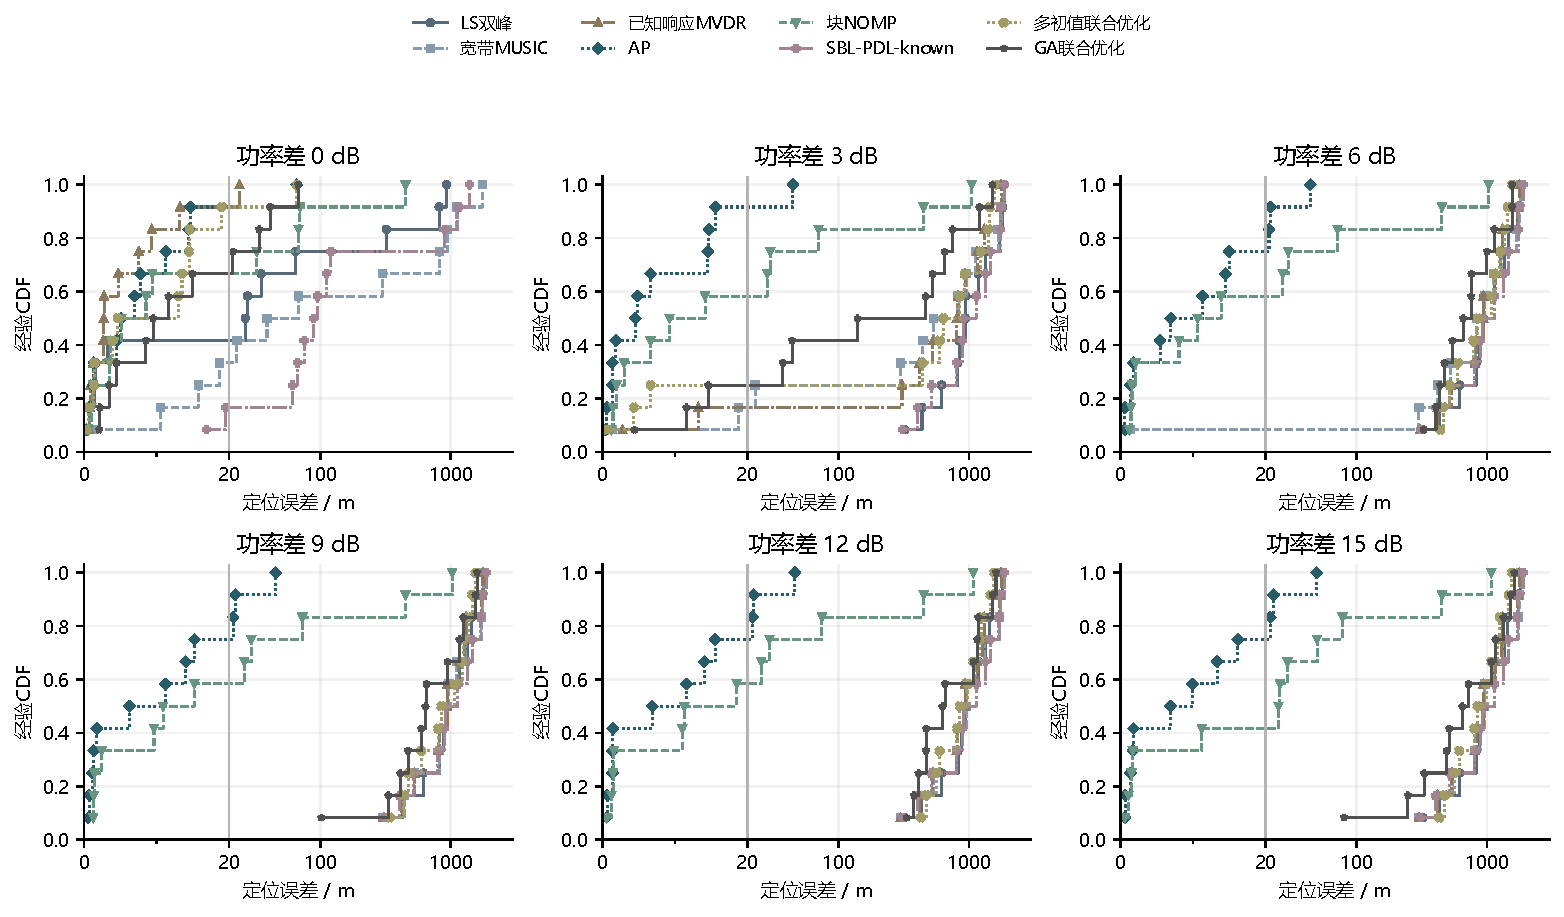
\includegraphics[width=\linewidth]{figures/g10_cdf_weak.pdf}
\caption{弱源误差CDF，坐标尺度与强源图一致。}\label{fig:g10-cdf-weak}\end{figure}

\subsection{早期估计、完整耗时与运算量}
\begin{figure}[htbp]\centering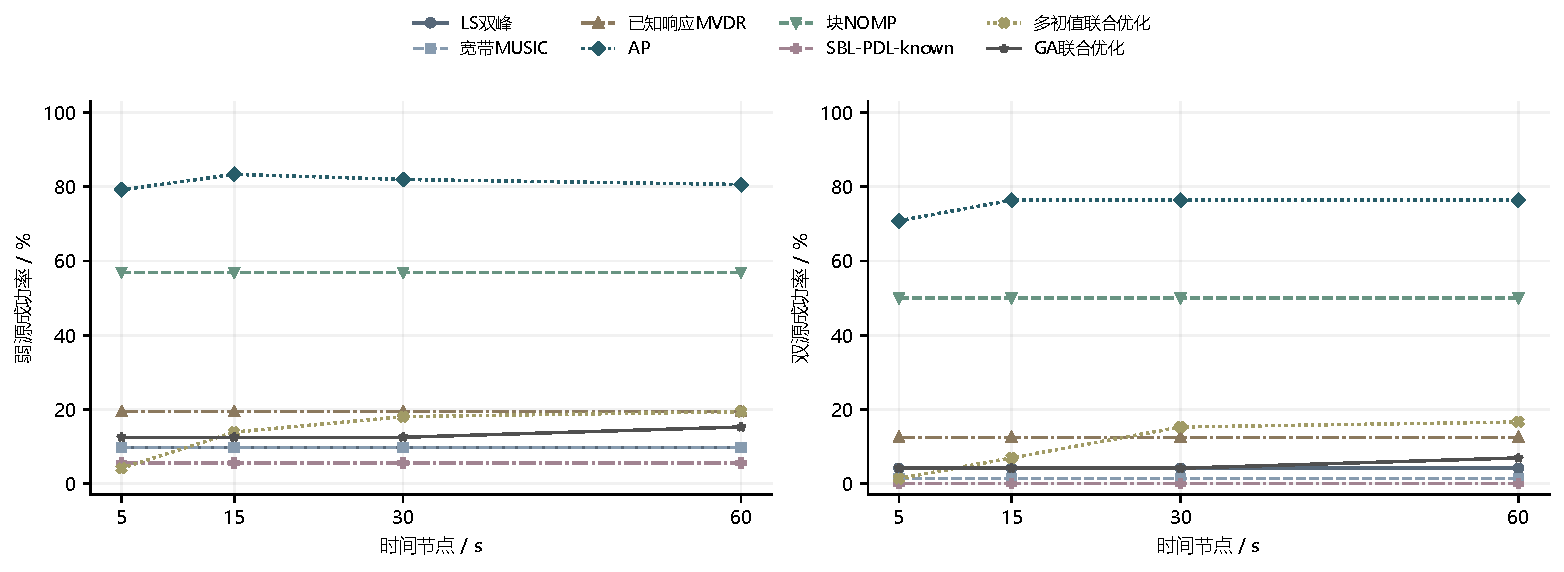
\includegraphics[width=\linewidth]{figures/g10_time.pdf}
\caption{共同时间节点下的定位成功率，每种方法包含72条混合记录。}\label{fig:g10-time}\end{figure}
AP在5 s节点已有57/72条弱源定位成功，15 s为60/72，30 s为59/72，60 s为58/72；对应双源成功数为51、55、55、55。AP保存联合残差更小的估计，但残差下降与真值误差下降并非逐样本一致。15 s以后强源RMSE继续下降，弱源成功数和RMSE则出现小幅变化。因此应分别考察获得较好估计的早期时间与完整搜索耗时。

\begin{figure}[htbp]\centering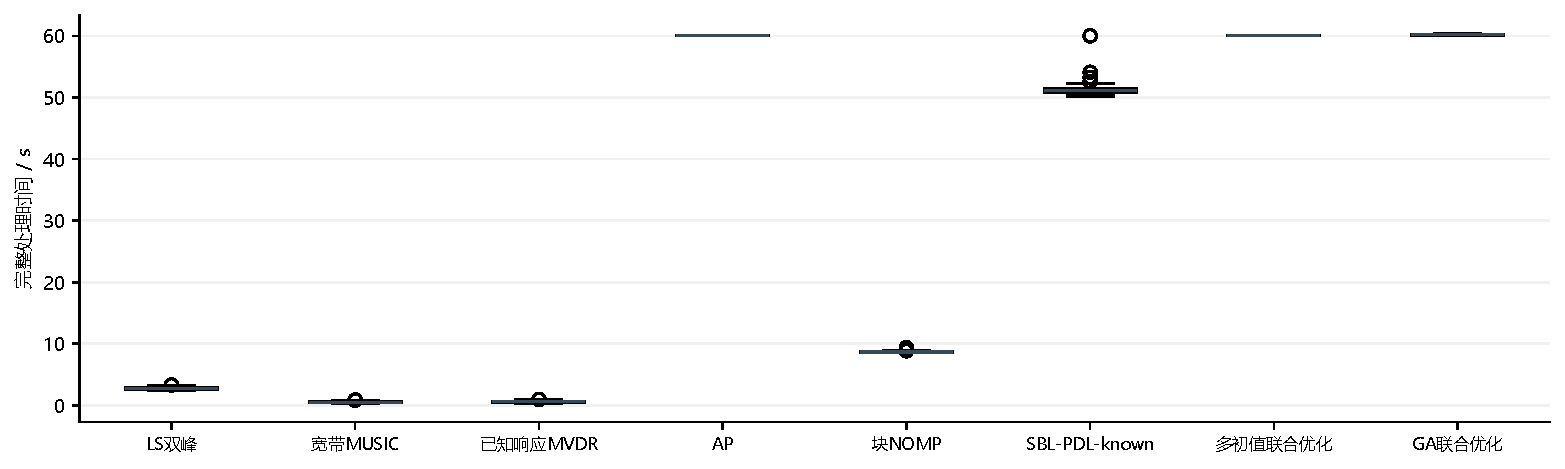
\includegraphics[width=\linewidth]{figures/g10_runtime.pdf}
\caption{72条混合记录的完整耗时分布。箱体为四分位范围，中线为中位数，须线采用1.5倍四分位距。}\label{fig:g10-runtime}\end{figure}
\begin{table}[htbp]\centering\small
\caption{混合源完整耗时与平均运算量}\label{tab:g10-cost}
\begin{tabular}{lrrrrr}\toprule
方法 & 中位数/s & 95\%分位/s & 响应点数/$10^9$ & 联合评价次数 & 协方差分解次数\\\midrule
LS双峰 & 2.71 & 3.05 & 0.677 & 0.0 & 0\\
宽带MUSIC & 0.53 & 0.76 & 0.044 & 0.0 & 4096\\
已知响应MVDR & 0.58 & 0.81 & 0.023 & 0.0 & 4096\\
AP & 60.05 & 60.10 & 1.187 & 532.9 & 0\\
块NOMP & 8.67 & 8.88 & 1.327 & 41.0 & 0\\
SBL-PDL-known & 51.17 & 52.40 & 2.785 & 0.0 & 1653646\\
多初值联合优化 & 60.06 & 60.10 & 0.185 & 542.9 & 0\\
GA联合优化 & 60.18 & 60.36 & 0.188 & 637.6 & 0\\
\bottomrule\end{tabular}
\end{table}
块NOMP平均完整耗时8.70 s，AP为60.06 s。前者较快结束，后者继续用剩余预算搜索和回访候选。表\ref{tab:g10-cost}同时给出响应计算点数、联合目标评价及协方差分解次数；不同方法的计算组织和每次评价内容不同，这些计数用于说明计算构成，实际代价以完整耗时为准。

\subsection{孤立源参照与困难布局}
\begin{figure}[htbp]\centering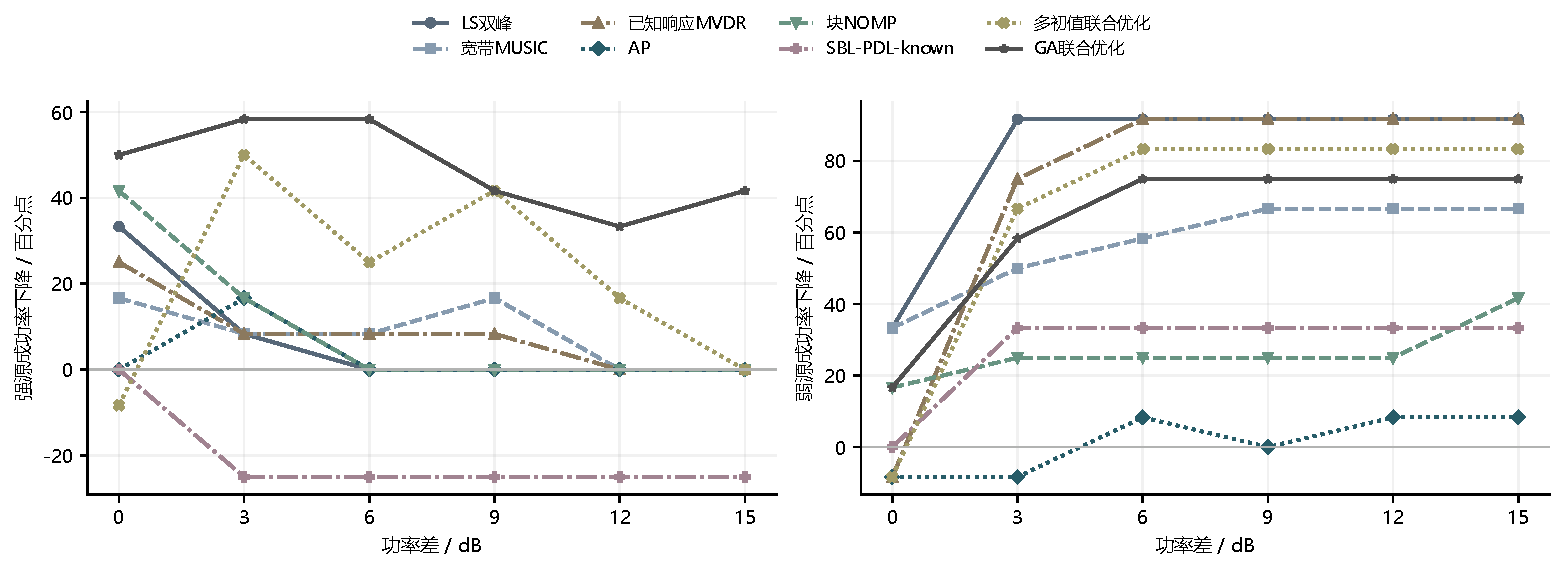
\includegraphics[width=\linewidth]{figures/g10_paired.pdf}
\caption{共同30 s节点下，孤立源成功率减去混合源成功率。正值表示加入另一源后成功率下降，每档均按12个布局配对。}\label{fig:g10-paired}\end{figure}
孤立弱源在LS、MUSIC、MVDR、AP、块NOMP、SBL、多初值和GA中的成功数依次为11、8、11、10、10、4、10、9（分母12）。在15 dB混合场景，相应弱源成功数为0、0、0、9、5、0、0、0。AP保留了大部分单源定位能力，块NOMP存在部分新增干扰损失。MUSIC和SBL的孤立强源成功数也分别为24/72和6/72，说明其本轮分段协方差与稀疏字典实现已有单源适配问题，混合表现需要结合这些参照理解。

AP在60 s节点的14次弱源失败集中于三个布局。以15 dB的30 s配对结果为例，这三个布局的孤立弱源误差约为2.75、21.60、26.32 m，混合弱源误差约为23.11、21.74、49.22 m。第一个布局新增阈值失败，第二个变化较小，第三个原已超过阈值且误差进一步增加。该配对关系区分了原有误差和强源加入后的损失，也提示后续应按布局研究耦合与搜索路径。

\subsection{代表性空间图}
图\ref{fig:g10-map0}--\ref{fig:g10-map15}使用预先选定的同一布局及同一组基础波形，分别展示0、9和15 dB。LS、MUSIC和MVDR为各自原生谱；SBL显示后验均值系数功率；AP、块NOMP、多初值与GA显示固定第一个估计位置后的条件LS切片。该切片反映另一候选位置的残差下降，并标明固定位置。

\begin{figure}[htbp]\centering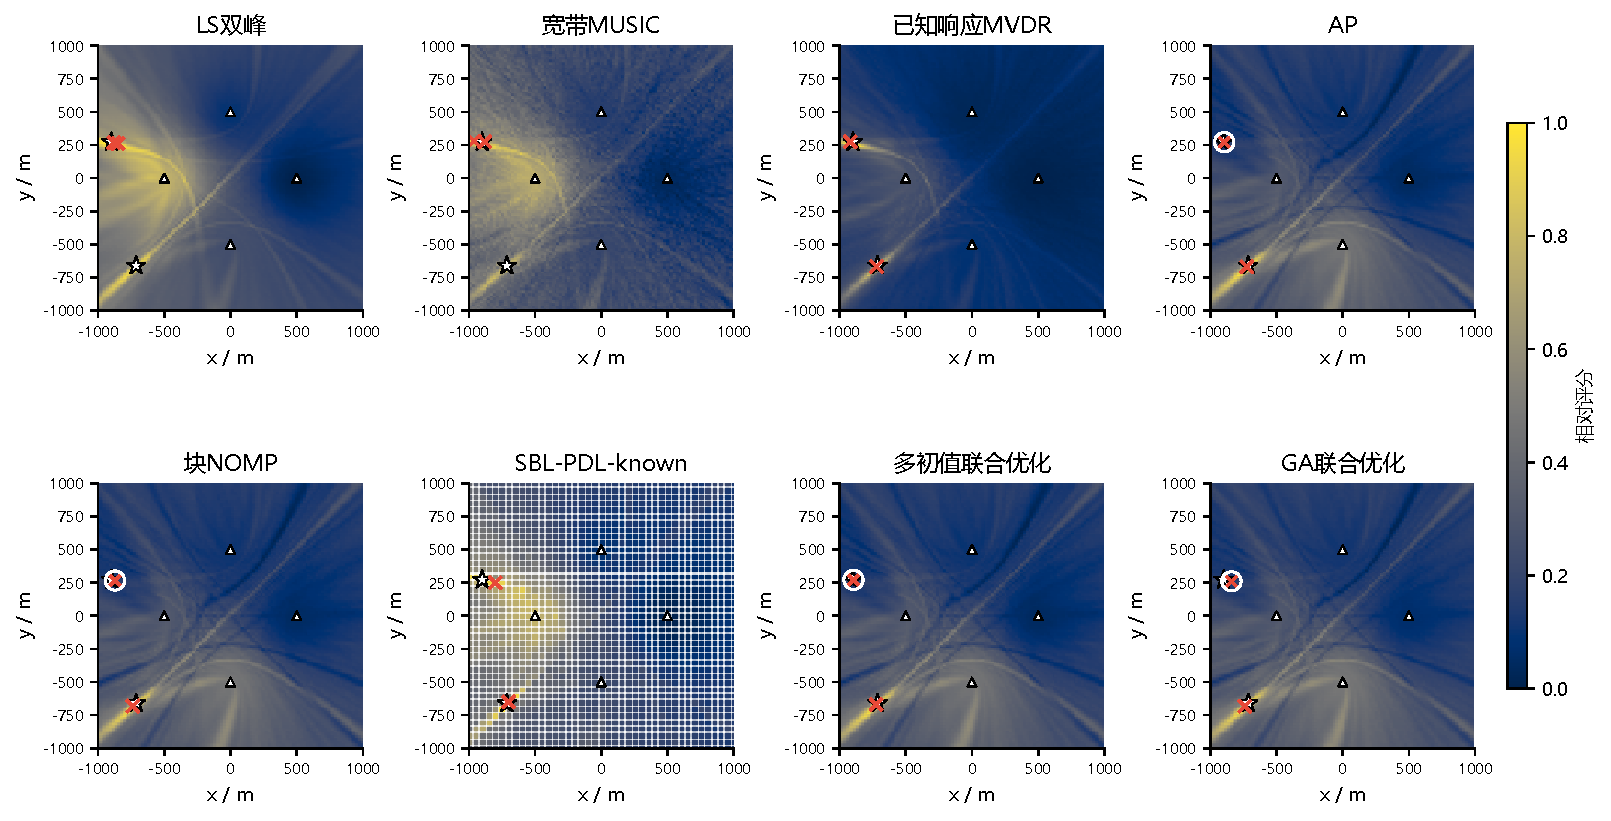
\includegraphics[width=\linewidth]{figures/g10_maps_0.pdf}
\caption{0 dB下八种方法的空间图。三角为站点，星号为真值，叉号为估计位置，空心圆为条件谱的固定位置。各面板按$(S-S_{\min})/(S_{\max}-S_{\min})$显示相对评分。}\label{fig:g10-map0}\end{figure}
\begin{figure}[htbp]\centering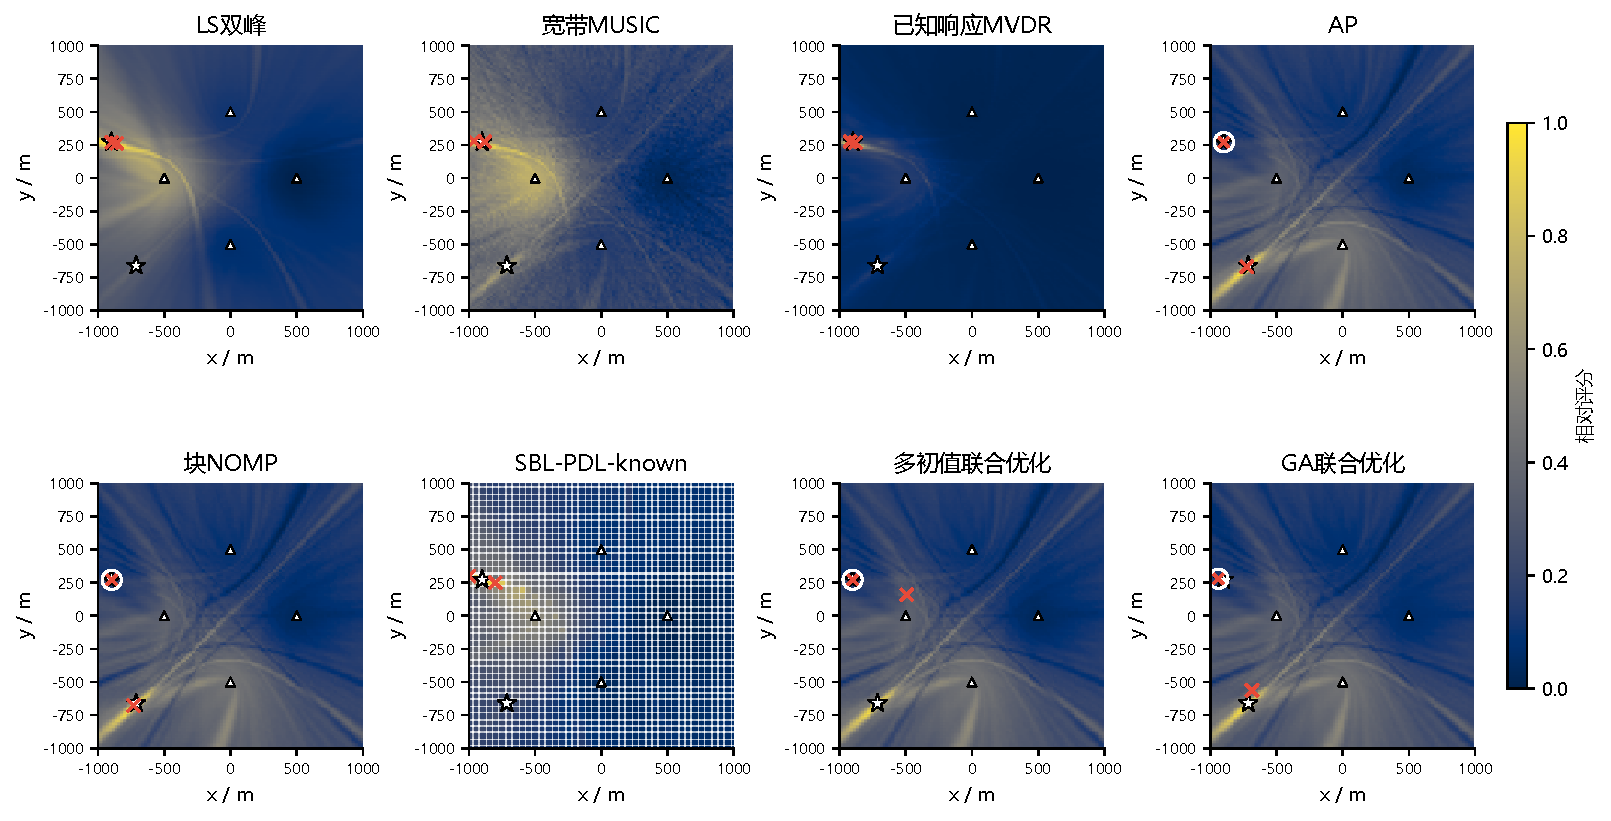
\includegraphics[width=\linewidth]{figures/g10_maps_9.pdf}
\caption{9 dB下的空间图。符号和归一化方式同图\ref{fig:g10-map0}。}\label{fig:g10-map9}\end{figure}
\begin{figure}[htbp]\centering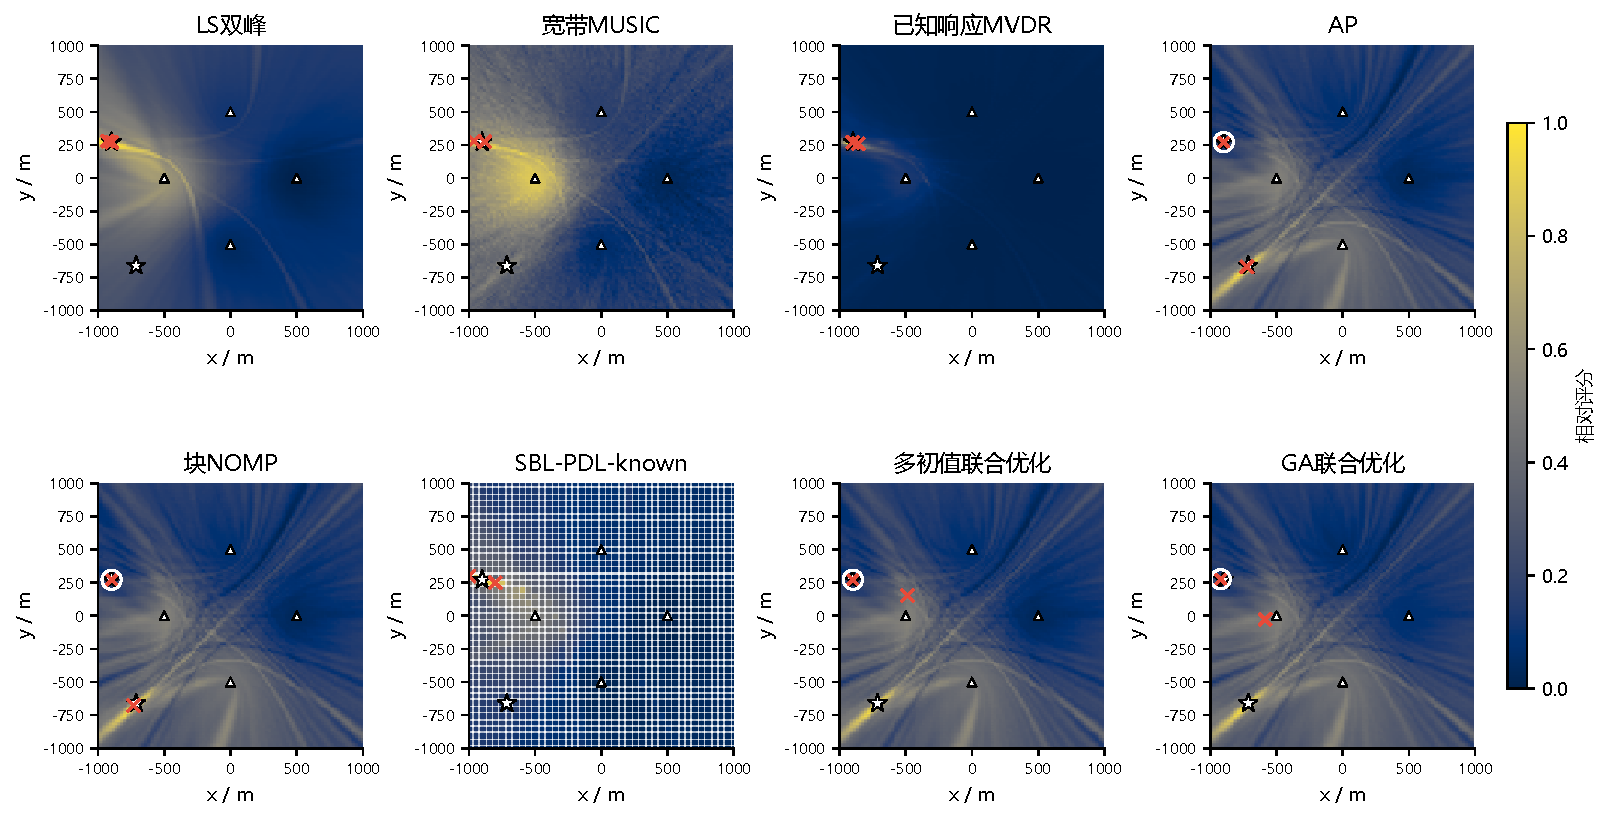
\includegraphics[width=\linewidth]{figures/g10_maps_15.pdf}
\caption{15 dB下的空间图。显示网格为20 m，SBL使用可局部移动的50 m字典点；估计标记来自连续位置输出。}\label{fig:g10-map15}\end{figure}
功率差增加后，单源扫描谱的显著峰更集中于强源附近。条件图则随已固定的估计位置变化；即使使用相同联合目标，不同搜索路径也可能得到不同切片。比较时同时观察真值附近的评分、最终估计和固定位置。空间图说明该代表性样本的定位过程，整体性能由前述12布局统计给出。

\section{讨论}\label{sec:new-discussion}
AP在较早时间节点获得了较高成功率，继续搜索主要改善联合拟合，弱源阈值成功数并未随之持续增加。后续可围绕候选排序、回访时机和停止条件分配计算，将早期有效搜索与后续收益较小的更新分开分析。

块NOMP以较少完整处理时间获得41/72的弱源成功数，但误差长尾仍较突出。AP与块NOMP在检测评分、循环更新和全局候选覆盖上不同；多初值与GA则从四维联合目标出发。下一步可在相同观测上追踪这些路径进入不同吸引域的过程，判断困难布局更需要候选覆盖还是联合位置调整。

MUSIC和SBL的单源参照偏低，首先需要检查短记录分段的子空间稳定性，以及字典间距、活动集选择和位置细化对单源估计的影响。当前结果已给出功率差增加时的退化现象，并显示AP和块NOMP具有不同的可靠性与耗时特点。是否提出新的定位方法，可在解决上述具体问题后进一步判断。
